\section{Thursday, March 23rd: Native vs Web Apps}
\subsection{Implementing Interfaces, Part 1}
We have talked about the design process as the cycle that happens in the red phase. In the programming assignments, you have been in the ``Engineering'' phase.

Before we got to GUIs, everyone interacted with computers through command-line prompts, a model where interaction is done via the system.

\subsubsection{Xerox Alto (1973)}
The system is waiting for an interaction and responds once that has happened. This was one of the first interactive programs.

One way you can do this is with a switch statement in an infinite while loop but this only works if your computer is only running 1 process. The reason for this is because they were written by different people.

\subsection{Native Apps: GUI Toolkits}
Today most native apps are written via toolkits such as QT, Cocoa, Java Swing, GTK, etc.

\subsection{Native Apps}
These are self-contained programs made to run directly on a target OS (Windows, Linux, MacOS, Andriod, iOS, etc).

There are a multitude of UI toolkits even if there is a `canonical' toolkit for the OS, and third-party toolkits can help you get closer to the platform-independence that web apps. However this has the cost of not looking like it was \textit{meant} for the current OS.

An advantage of Toolkits over Web Apps is that they are generally quicker in updating to allow using new hardware.

Note that Programming Language is orthogonal to the toolkit. You can use almost any language for almost any toolkit.
\begin{important}
This means that you will have to have an `Android Team' and an `iOS Team' -- even if you share some code, the frontend UI will be split across 2 codebases with completely different code.
\end{important}

\subsubsection{Android SDK Example}
- Highest Level\\
View Class\\
Activity System\\
Native Libraries + Android Runtime\\
Linux Kernel\\
- Lowest Level

\subsection{Web Apps}
This semester we are working on web applications which are delivered by a \textit{web server} and run on a \textit{web browser}.

\begin{shaded}
A \textit{Client} requests resources from  server.
\end{shaded}

\begin{shaded}
A \textit{Server} transfers data for UI and interaction logic to client.
\end{shaded}

\begin{shaded}
A \textit{Browser} on the client parses received data, builds \& renders the UI and processes user input events
\end{shaded}

You can refer to names in the DOM in JavaScript -- a language for defining interactive behavior.

Note that with different OS/vendors, you may see some slight differences.

There are Pros/Cons to using Web \& Native Apps and these can be seen in the table in lecture slides.

\subsection{Disentangling}
We usually separate HTML DSL from CSS/JS code.

Instead of using \texttt{<style>} and \texttt{<script>} tags, we designate explicit \texttt{.css} and \texttt{.js} files for CSS \& JavaSctipt code respectively.

\subsection{DOM (Document Object Model)}
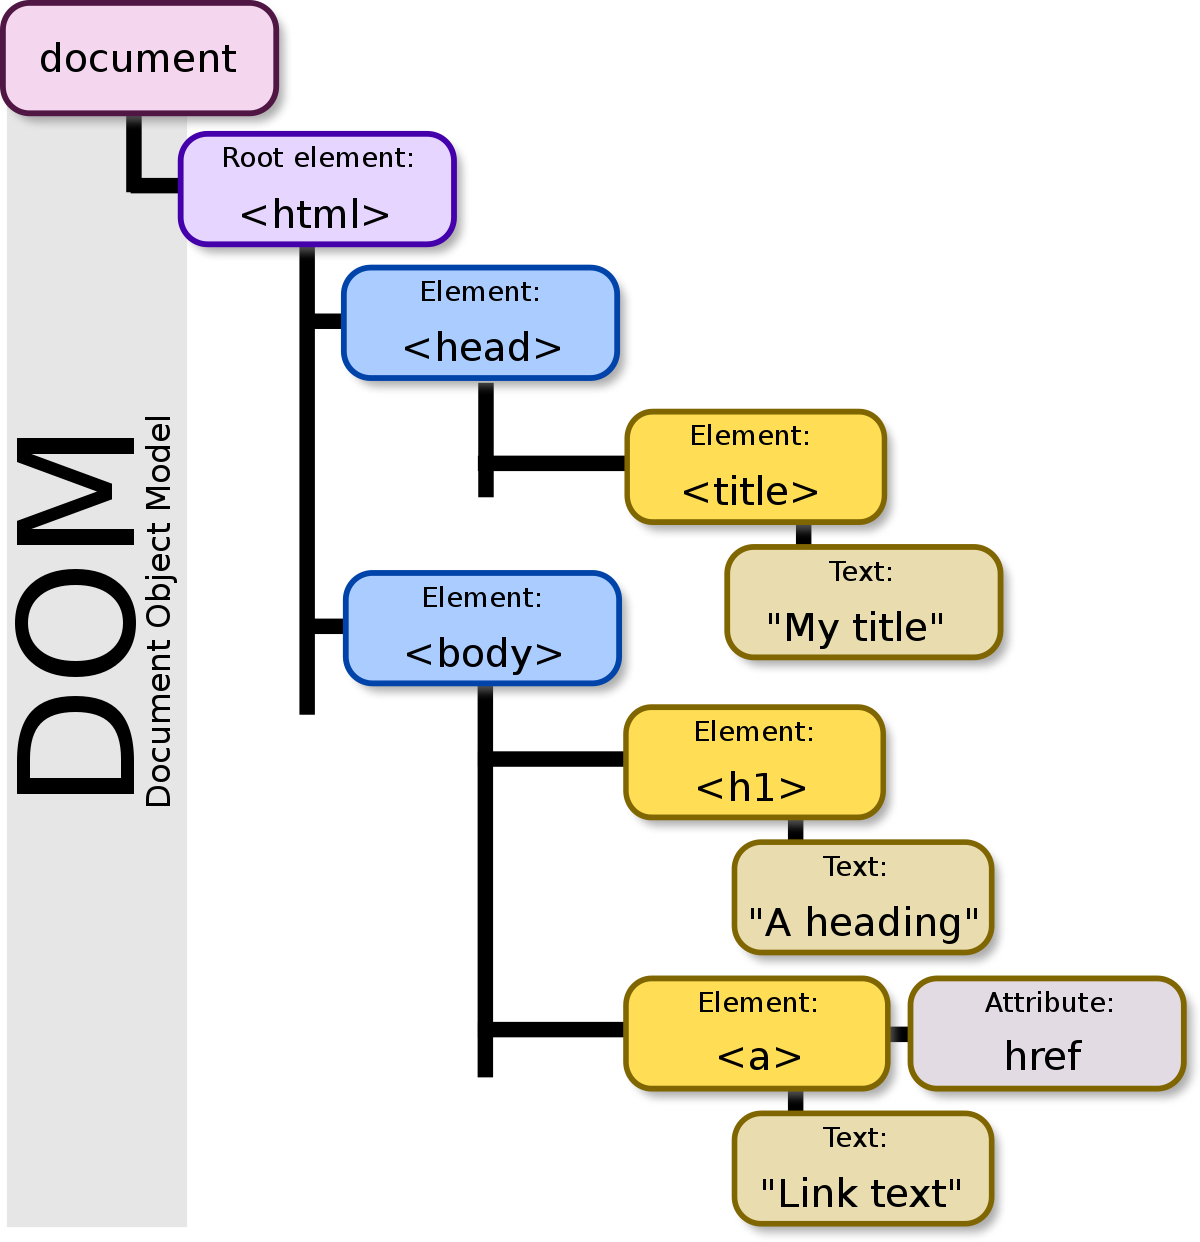
\includegraphics[scale=0.15]{lectures/wk10/dom.png}

\subsection{Web App with server-side code}
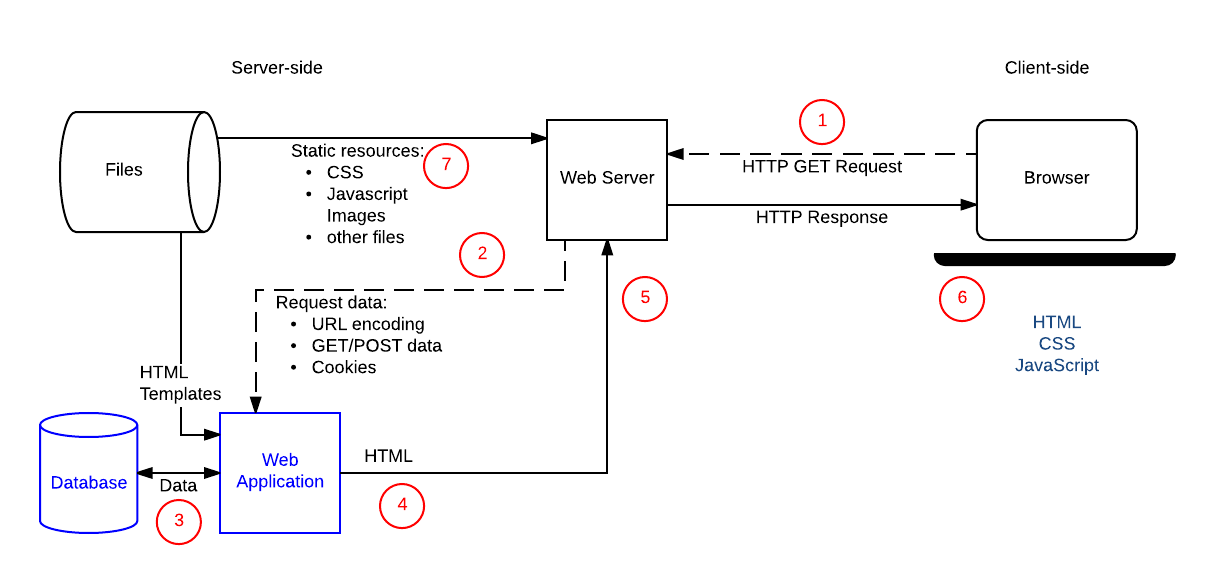
\includegraphics[scale=0.75]{lectures/wk10/web_app.png}


\subsection{Client-side Web Frameworks}
HTML was made for \textit{Documents} -- not UI.
\begin{itemize}
    \item React JS (Facebook)
    \item Angular JS (Google)
    \item JQuery
\end{itemize}
Note that JQuery is still considered a Client-side Web Framework even though it does not really change how your server communicates like the others.

